\documentclass[12pt]{beamer}
\usepackage{beamerthemeHannover, graphicx, clrscode, amsmath, amssymb, multicol}
\usepackage{verbatim}
\setbeamercolor{sidebar}{use=structure,bg=gray!60!green}
\title{ Slicing and Dicing Plant Genomes with Perl }
\author[@dukeleto]{Jonathan "Duke" Leto \\ Sol Genomics Network \\ http://solgenomics.net }
\date{}

\begin{document}

\frame{
    \titlepage
    \begin{center}
    
\includegraphics[scale=0.5]{sgn_logo}
    \end{center}
}

\frame{
    \frametitle{What is Sol Genomics Network? (SGN)}

    SGN is an NSF-funded Model Organism Database on the web.  \\

    \begin{itemize}
    \item A model organism is a species that is extensively studied to understand
    particular biological phenomena, with the expectation that discoveries made
    in the organism model will provide insight into the workings of other
    organisms.
    \end{itemize}
}

\frame{
    \frametitle{What is Sol Genomics Network? (Continued)}

    SGN is part of the Lukas Mueller research lab at Boyce Thompson Institute
    for Plant Research (BTI), located on the Cornell University campus. \\

    \begin{center}
    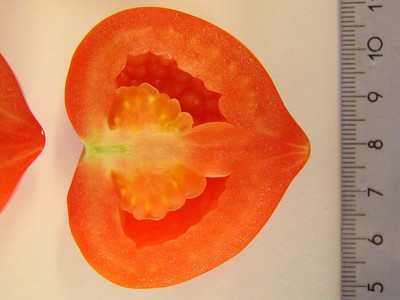
\includegraphics[scale=0.3]{tomato}
    \end{center}

    We study the Solanaceae (Nightshade family): Tomato, Potato, Petunia, Eggplant, and many more
}

\frame{
    \frametitle{Who uses SGN?}
    \begin{itemize}
        \item Evolutionary plant biologists
        \item Plant biochemists
        \item Plant disease researchers
        \item Plant breeders
    \end{itemize}
    \begin{center}
    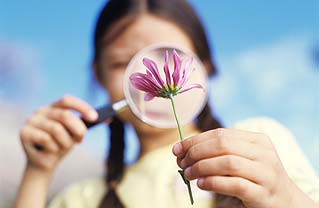
\includegraphics[scale=0.7]{plant-study}
    \end{center}
}

\frame{
    \frametitle{Code By Numbers}

    Every line of code goes on Github, anything reusable goes to CPAN. \\

    \begin{itemize}
        \item 29 public Github repos
        \item 10 committers
        \item $\sim$ 10 CPAN modules released (more on the way)
        \item Over 200K lines of Perl
        \begin{itemize}
            \item Lots of legacy code, slowly modernizing
            \item Converted to Catalyst last year
        \end{itemize}
    \end{itemize}
}

\frame{
    \frametitle{Some CPAN Modules}
    \begin{itemize}
        \item Bio::Chado::Schema - DBIx::Class schema for Chado
        \item Bio::GFF3 - Manipulate GFF3 data files
        \item Bio::Blast - Interact with BLAST databases
        \item Catalyst::View::Bio::Seqio - Catalyst view for Bioperl sequences
        \item Yapri - Yet Another Perl R Interface
    \end{itemize}
}

\frame{
    \frametitle{What we depend on most}
    \begin{itemize}
        \item Moose
        \item Catalyst
        \item DBIx::Class
        \item Plack
        \item Starman
        \item BioPerl
        \item Mason
        \item WWW::Mechanize
        \item autodie
        \item Test::*
    \end{itemize}
}

\frame{
    \frametitle{My current project}
    Mimosa: Miniature Model Organism Sequence Aligner \\

    \begin{center}
    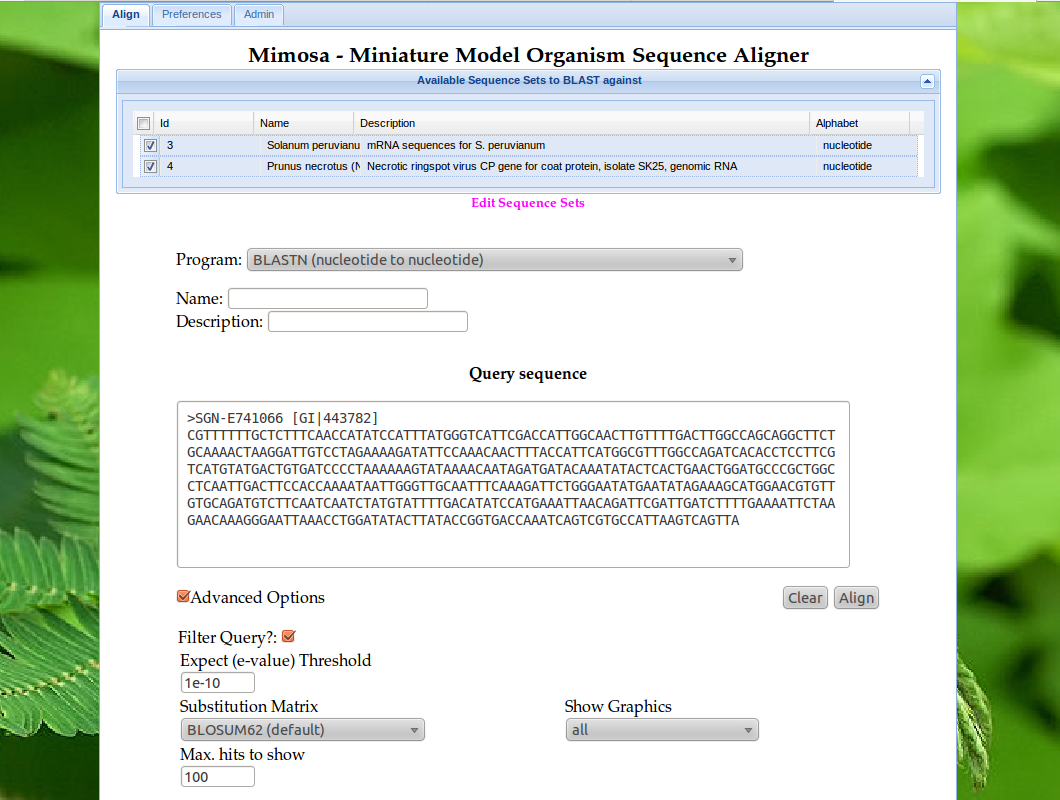
\includegraphics[scale=0.3]{mimosa2}
    \end{center}

    Web interface to not-so-friendly command-line utilities for evolutionary biologists
}

\frame{
    \frametitle{ Resources }
    \begin{center}
        \begin{itemize}
           \item http://solgenomics.net
           \item http://github.com/solgenomics
           \item \#cxgn on irc.perl.org
        \end{itemize}
    \end{center}
}

\frame{
    \frametitle{ Thanks! }
    \begin{itemize}
        \item Boyce Thompson Institute for Plant Research
        \item National Science Foundation
        \item All the Perl + CPAN hackers that make SGN possible
    \end{itemize}

    \begin{center}
    
\includegraphics[scale=1.0]{tomato_happy}
    \end{center}
}

\end{document}
